\documentclass[11pt,a4paper]{article}

% -------------------------------------------------
% Packages
% -------------------------------------------------
\usepackage[margin=1in]{geometry}
\usepackage[T1]{fontenc}
\usepackage[utf8]{inputenc}
\usepackage{lmodern}
\usepackage{microtype}
\usepackage{amsmath,amssymb}
\usepackage{booktabs}
\usepackage{longtable}
\usepackage{array}
\usepackage{caption}
\usepackage{xcolor}
\usepackage{graphicx}
\usepackage{float}
\usepackage{fancyhdr}
\usepackage{lastpage}
\usepackage{titlesec}
\usepackage{enumitem}
\usepackage[hidelinks]{hyperref}
\usepackage{pgfplots}
\pgfplotsset{compat=1.18}

% -------------------------------------------------
% Page style
% -------------------------------------------------
\pagestyle{fancy}
\fancyhf{}
\fancyhead[L]{Packet Sniffing Report}
\fancyhead[R]{Internet of Things -- IoT Challenge \#2}
\renewcommand{\headrulewidth}{0.4pt}
\renewcommand{\footrulewidth}{0pt}
\fancyfoot[C]{\thepage/\pageref{LastPage}}

% -------------------------------------------------
% Section formatting
% -------------------------------------------------
\titleformat{\section}{\normalfont\large\bfseries}{\thesection.}{0.5em}{}
\titleformat{\subsection}{\normalfont\normalsize\bfseries}{}{0em}{}
\setlist[itemize]{leftmargin=1.5em}
\setlength{\parskip}{0.4em}
\setlength{\parindent}{0pt}

% -------------------------------------------------
% Document
% -------------------------------------------------
\begin{document}

\begin{center}
    {\LARGE \textbf{Packet Sniffing Report}}\\[0.4em]
    {\large Internet of Things -- IoT Challenge \#2}\\[1.2em]
    Mobin Khatib - 11114435\\
    Ali Edareh Heidarabadi - 11036028\\[0.6em]
    Politecnico di Milano\\[0.6em]
    April 23, 2026
\end{center}

\vspace{1em}

\begin{abstract}
This report presents the solution to Part 1 of the challenge, namely questions CQ1--CQ8 on the packet captures \texttt{A.pcapng} and \texttt{B.pcapng}. Malformed packets were ignored, consistently with the assignment statement. The final counts were obtained through script-based analysis and then checked manually in Wireshark, with particular attention to CoAP request--response matching, Observe notifications, MQTT-SN decoding on UDP port 1885, wildcard subscriptions, retained-message deletions, and topic-depth extraction for local-broker publish traffic.
\end{abstract}

\section*{Methodology and interpretation rules}
The analysis was carried out with a protocol-aware workflow. CoAP, MQTT, MQTT-SN, and related auxiliary traffic were parsed programmatically so that retransmissions, acknowledgments, retained publishes, wildcard topic filters, and client identifiers could be handled consistently. Wireshark was then used for manual spot checks on the most delicate cases.

Three interpretation rules are especially important for the final results. First, in CQ1b, a DELETE request is considered successful only if the resource is verifiably absent afterwards; a positive status code alone is not sufficient. Second, in CQ3a, the initial piggybacked Observe response is not counted as a separate notification. Third, in CQ6a, every retained PUBLISH with zero-byte payload is counted as an erasure event, following the convention clarified in the forum.

\section*{Summary of final answers}
Table~\ref{tab:summary} collects the final answers in compact form.

\begin{table}[H]
\centering
\caption{Final answers for CQ1--CQ8.}
\label{tab:summary}
\small
\begin{tabular}{>{\raggedright\arraybackslash}p{0.12\textwidth} >{\raggedright\arraybackslash}p{0.12\textwidth} >{\raggedright\arraybackslash}p{0.66\textwidth}}
\toprule
\textbf{Question} & \textbf{Answer} & \textbf{Brief justification} \\
\midrule
CQ1a & 1 (MID 30800) & Exactly one NON-confirmable CoAP DELETE directed to \texttt{coap.me} received a successful response. \\
CQ1b & 0 & A subsequent GET still returned 2.05 Content, so the resource was not actually removed. \\
CQ2 & 1 (\texttt{/dining\_room}) & Only one local CoAP resource had equal positive counts of unique unsuccessful CON POST and CON PUT requests. \\
CQ3a & 10 & Only separate Observe notifications were counted; the initial piggybacked reply was excluded and retransmissions were ignored. \\
CQ3b & 5 & Five Confirmable notifications were sent after the client had become unreachable and never received an ACK. \\
CQ4 & 0 & The apparent MQTT-SN deliveries failed at the IP layer, so no client actually received a broker message. \\
CQ5 & 1 & Only one subscriber received a Last Will message due to a wildcard-based subscription. \\
CQ6a & 5 & Five distinct HiveMQ clients published at least one zero-byte retained message. \\
CQ6b & 2 & Two of those five clients used identifiers longer than 7 bytes. \\
CQ7 & 9 & Nine SUBSCRIBE requests to the local broker contained a topic filter with at least two wildcards. \\
CQ8a & 439 & Total number of local-broker PUBLISH messages considered in \texttt{A.pcapng}. \\
CQ8b & 534 & Total number of local-broker PUBLISH messages considered in \texttt{B.pcapng}. \\
\bottomrule
\end{tabular}
\end{table}

\section*{Question-by-question discussion}

\subsection*{CQ1a -- Successful NON-confirmable DELETE requests to \texttt{coap.me}}

\textbf{Final answer:} 1 request, with MID 30800.

\paragraph{Motivated response.}
I selected all CoAP DELETE requests sent as NON messages to \texttt{coap.me}
(\texttt{134.102.218.18:5683}) and checked whether they received a successful CoAP response.
Using the notebook code, requests were matched with replies through the same CoAP token.
Exactly one request satisfies all conditions, and its MID is \textbf{30800}.

\paragraph{Filters used.}
\begin{verbatim}
coap && ip.dst == 134.102.218.18 && udp.dstport == 5683 &&
coap.type == 1 && coap.code == 4
\end{verbatim}

\paragraph{Additional code / comments.}
A short Python script was used to parse the trace, match each request with the first later
reverse-direction response having the same token, and count only responses in the CoAP
success class (2.xx, i.e. code 64--95).

\begin{verbatim}
for request in events:
    if (request["type"] == 1 and request["code"] == 4 and
        request["dst"] == COAP_ME_IP and request["dport"] == COAP_PORT):
        for response in events:
            if (response["ts"] > request["ts"] and
                response["src"] == request["dst"] and
                response["dst"] == request["src"] and
                response["token"] == request["token"]):
                if 64 <= response["code"] < 96:
                    successful_requests.append((request, response))
                break
\end{verbatim}
\subsection*{CQ1b -- Requests that actually achieved the desired outcome}

\textbf{Final answer:} 0.

\paragraph{Motivated response.}
The DELETE request from CQ1a receives a \texttt{2.02 Deleted} response, but this is not enough
to prove that the resource was really removed. The notebook checks whether a later GET to the
same URI still succeeds. Since a subsequent GET returns \texttt{2.05 Content}, the resource
still exists. Therefore, no request actually achieved the desired outcome.

\paragraph{Filters used.}
\begin{verbatim}
coap.code == 4
coap.code == 1
\end{verbatim}

\paragraph{Additional code / comments.}
The notebook extracts the URI of the DELETE request, then checks for a later GET to the same
resource. If the GET reply is \texttt{2.05 Content}, the deletion is not counted as successful.

\begin{verbatim}
if response["code"] == 66:  # 2.02 Deleted
    target_uri = get_uri_path(request["options"])
    for later_req in events:
        if later_req["ts"] > response["ts"] and later_req["code"] == 1 \
           and get_uri_path(later_req["options"]) == target_uri:
            for later_resp in events:
                if later_resp["ts"] > later_req["ts"] and \
                   later_resp["token"] == later_req["token"]:
                    if later_resp["code"] == 69:  # 2.05 Content
                        resource_still_exists = True
                    break
\end{verbatim}
\subsection*{CQ2 -- Resources with equal numbers of unsuccessful CON POST and PUT requests}

\textbf{Final answer:} 1 resource, namely \texttt{/dining\_room}.

\paragraph{Motivated response.}
For each resource on the local CoAP server, I counted unique unsuccessful Confirmable POST
requests and unique unsuccessful Confirmable PUT requests separately. A request was counted
as unsuccessful only if it received an explicit non-success response. With this rule, only
\texttt{/dining\_room} has equal positive counts for both classes.

\paragraph{Filters used.}
\begin{verbatim}
coap.type == 0 && coap.code == 2
coap.type == 0 && coap.code == 3
\end{verbatim}

\paragraph{Additional code / comments.}
The notebook matches each CON POST/PUT request with its reply, keeps only explicit
non-success responses, groups requests by URI, and compares the two counters.

\begin{verbatim}
if req["type"] == 0 and req["code"] in (2, 3):   # CON POST / PUT
    if resp is not None and not (64 <= resp["code"] < 96):
        uri = get_uri_path(req["options"])
        if req["code"] == 2:
            bad_post[uri].add(req["mid"])
        else:
            bad_put[uri].add(req["mid"])
\end{verbatim}
\subsection*{CQ3a -- Separate Observe notifications for \texttt{/dining\_room/temperature}}

\textbf{Final answer:} 10.

\paragraph{Motivated response.}
The word \emph{separate} is important here. The initial piggybacked reply used to establish the
Observe relationship is not counted as a separate notification, so frame 4344 is excluded.
After removing retransmissions, the remaining separate Observe notifications are exactly
\textbf{10}.

\paragraph{Filters used.}
\begin{verbatim}
coap.observe
\end{verbatim}

\paragraph{Additional code / comments.}
The notebook removes the initial piggybacked response and ignores retransmissions before
counting the remaining Observe notifications.

\begin{verbatim}
if is_observe_notification(pkt) and pkt["frame_no"] != 4344:
    if not is_retransmission(pkt):
        notifications.append(pkt)
\end{verbatim}
\subsection*{CQ3b -- Useless notifications}

\textbf{Final answer:} 5.

\paragraph{Motivated response.}
I interpreted useless traffic at the network level. A notification is counted as useless when it is
sent even though it can no longer be meaningfully delivered to the observer. In the trace, the
server keeps sending five Confirmable notifications after the client becomes unreachable, and
none of them is acknowledged. Therefore, the number of useless notifications is \textbf{5}.

\paragraph{Filters used.}
\begin{verbatim}
coap.type == 0
\end{verbatim}

\paragraph{Additional code / comments.}
The notebook selects Confirmable notifications sent after the client becomes unreachable and
counts only those that do not receive an ACK.

\begin{verbatim}
if pkt["type"] == 0 and is_observe_notification(pkt):
    if client_unreachable and not has_ack(pkt):
        useless_notifications.append(pkt)
\end{verbatim}
\subsection*{CQ4 -- MQTT-SN messages received by clients from the local broker}

\textbf{Final answer:} 0.

\paragraph{Motivated response.}
After enabling MQTT-SN dissection on UDP port \texttt{1885}, the broker-to-client packets can
be identified correctly. However, these transmissions are accompanied by ICMP Destination
Unreachable messages, which means the datagrams are not delivered at IP level. Therefore, the
number of MQTT-SN messages actually received by the clients is \textbf{0}.

\paragraph{Filters used.}
\begin{verbatim}
udp.port == 1885
icmp
\end{verbatim}

\paragraph{Additional code / comments.}
The notebook was used to identify valid MQTT-SN packets involving port \texttt{1885}. The final
answer was then refined by checking in Wireshark that the broker-to-client transmissions are
followed by ICMP Destination Unreachable messages, so they cannot be counted as received.
\subsection*{CQ5 -- Subscribers receiving a Last Will through a wildcard subscription}

\textbf{Final answer:} 1 subscriber.

\paragraph{Motivated response.}
I identified the clients subscribed with at least one wildcard and then checked which of them
received a Last Will publication. Only the client \texttt{zmjnxudohrkaegmh} satisfies both
conditions. Therefore, the number of subscribers is \textbf{1}.

\paragraph{Filters used.}
\begin{verbatim}
mqtt.msgtype == 8
mqtt.msgtype == 3
\end{verbatim}

\paragraph{Additional code / comments.}
The notebook matches wildcard subscriptions with received Last Will messages and counts the
distinct subscribers.

\begin{verbatim}
if is_wildcard_subscription(sub) and receives_last_will(sub.client_id, publishes):
    matched_subscribers.add(sub.client_id)
\end{verbatim}
\subsection*{CQ6a -- Clients that erased a retained value on HiveMQ}

\textbf{Final answer:} 5 clients.

\paragraph{Motivated response.}
Following the forum clarification, every retained PUBLISH with zero-byte payload is treated as
an erasure event, even if no retained value was previously stored on that topic. Counting the
distinct clients that perform at least one such operation gives \textbf{5} clients.

\paragraph{Filters used.}
\begin{verbatim}
mqtt.msgtype == 3
\end{verbatim}

\paragraph{Additional code / comments.}
The notebook selects retained PUBLISH messages with empty payload and counts the distinct
client identifiers that generated them.

\begin{verbatim}
if pkt["msgtype"] == 3 and pkt["retain"] == 1 and len(pkt["payload"]) == 0:
    erasing_clients.add(pkt["client_id"])
\end{verbatim}
\subsection*{CQ6b -- Clients with identifier length greater than 7 bytes}

\textbf{Final answer:} 2.

\paragraph{Motivated response.}
Among the five clients identified in CQ6a, I checked the CONNECT messages sent to the public
HiveMQ broker and measured the length of each client identifier. Exactly two of those clients
use an identifier with length strictly greater than 7 bytes.

\paragraph{Filters used.}
\begin{verbatim}
mqtt.msgtype == 1
\end{verbatim}

\paragraph{Additional code / comments.}
The notebook takes the set of clients found in CQ6a, extracts their client identifiers from the
CONNECT packets, and counts those with length greater than 7.

\begin{verbatim}
if pkt["msgtype"] == 1 and pkt["client_id"] in erasing_clients:
    if len(pkt["client_id"]) > 7:
        long_id_clients.add(pkt["client_id"])
\end{verbatim}
\subsection*{CQ7 -- SUBSCRIBE requests with at least two wildcards}

\textbf{Final answer:} 9.

\paragraph{Motivated response.}
The count is performed on MQTT SUBSCRIBE requests, not on unique clients or unique topic
filters. In \texttt{B.pcapng}, I selected SUBSCRIBE messages sent to the local broker and checked
whether at least one requested topic filter contains two or more wildcard symbols. This gives
a total of \textbf{9} requests.

\paragraph{Filters used.}
\begin{verbatim}
mqtt.msgtype == 8
\end{verbatim}

\paragraph{Additional code / comments.}
The notebook parses each SUBSCRIBE request, inspects all topic filters it contains, and counts
the request if any filter has at least two wildcard characters.

\begin{verbatim}
if pkt["msgtype"] == 8:
    for topic in pkt["topics"]:
        if topic.count("#") + topic.count("+") >= 2:
            matching_subscribes.append(pkt)
            break
\end{verbatim}
\subsection*{CQ8 -- Topic-layer histogram for local-broker publishes}

\textbf{Final answer:} CQ8a = 439 and CQ8b = 534.

\paragraph{Motivated response.}
I considered MQTT PUBLISH messages directed to the local broker and counted the number of
topic layers for each message. The corrected histogram is reported in Table~\ref{tab:cq8}.
Summing the histogram entries gives \textbf{439} messages for dataset A and \textbf{534}
messages for dataset B. No topic deeper than four layers appears in the corrected result.

\paragraph{Filters used.}
\begin{verbatim}
mqtt.msgtype == 3
\end{verbatim}

\paragraph{Additional code / comments.}
The notebook extracts each PUBLISH topic, computes its depth from the number of topic
segments, and updates the histogram for each dataset.

\begin{verbatim}
if pkt["msgtype"] == 3 and is_local_broker(pkt):
    depth = len([x for x in pkt["topic"].split("/") if x])
    hist[depth] += 1
\end{verbatim}

\begin{table}[H]
\centering
\caption{Corrected histogram data for CQ8.}
\label{tab:cq8}
\begin{tabular}{cccc}
\toprule
\textbf{Layer depth} & \textbf{Dataset A} & \textbf{Dataset B} & \textbf{Difference (B--A)} \\
\midrule
1 & 0   & 21  & 21 \\
2 & 154 & 172 & 18 \\
3 & 131 & 162 & 31 \\
4 & 154 & 179 & 25 \\
\midrule
Total & 439 & 534 & 95 \\
\bottomrule
\end{tabular}
\end{table}

\begin{figure}[H]
\centering
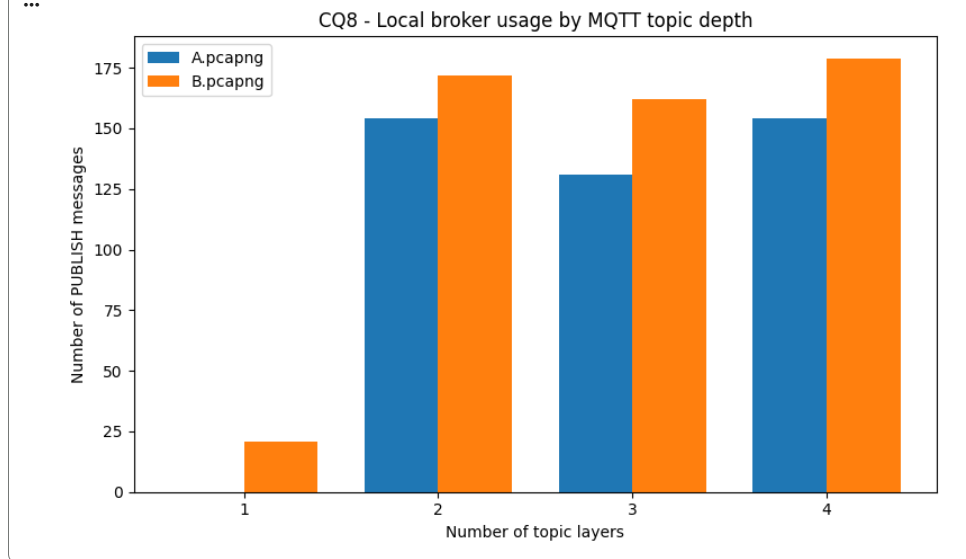
\includegraphics[width=0.78\textwidth]{1.png}
\caption{Histogram of MQTT topic depth for PUBLISH messages directed to the local broker.}
\label{fig:cq8}
\end{figure}
\section*{Notes on the analysis notebook}
The accompanying notebook automates the parsing of both packet captures and implements dedicated routines for each challenge question. In particular, it groups CoAP requests and responses so that retransmissions and piggybacked Observe replies are treated correctly, reconstructs MQTT sessions to analyze client identifiers, wildcard subscriptions, Last Will delivery, and retained-message erasures, and extracts publish-topic depth from all messages directed to the local broker in order to produce a reproducible CQ8 histogram.

This script-based workflow reduces ambiguity in the counting process and keeps the final answers consistent with the interpretation rules adopted in the report.

\section*{Conclusion}
The final solution becomes unique and reproducible once the main interpretation choices are stated explicitly. The most relevant ambiguities concern the stronger notion of success in CQ1b, the network-level meaning of useless traffic in CQ3b, and the zero-byte retained-publish convention used in CQ6a. With these conventions fixed, the answer set reported in Table~\ref{tab:summary} is internally consistent and suitable for submission.

\end{document}
